\documentclass{standalone}
\usepackage{tikz}

% Color Definitions
\definecolor{SourceColor}{RGB}{85,168,104}
\definecolor{TargetColor}{RGB}{221,132,82}
\definecolor{TargetChangerColor}{RGB}{255,153,0}
\definecolor{AbsorbingAreaColor}{RGB}{196,78,82}
\definecolor{ObstacleColor}{RGB}{179,179,179}
\definecolor{StairColor}{RGB}{129,114,178}
\definecolor{MeasurementAreaColor}{RGB}{255,0,0}
\definecolor{AgentColor}{RGB}{76,114,202}
\definecolor{AgentIdColor}{RGB}{255,127,0}

\newcommand{\MeasurementAreaOpacity}{0.549020}

\begin{document}
% Change scaling to [x=1mm,y=1mm] if TeX reports "Dimension too large".
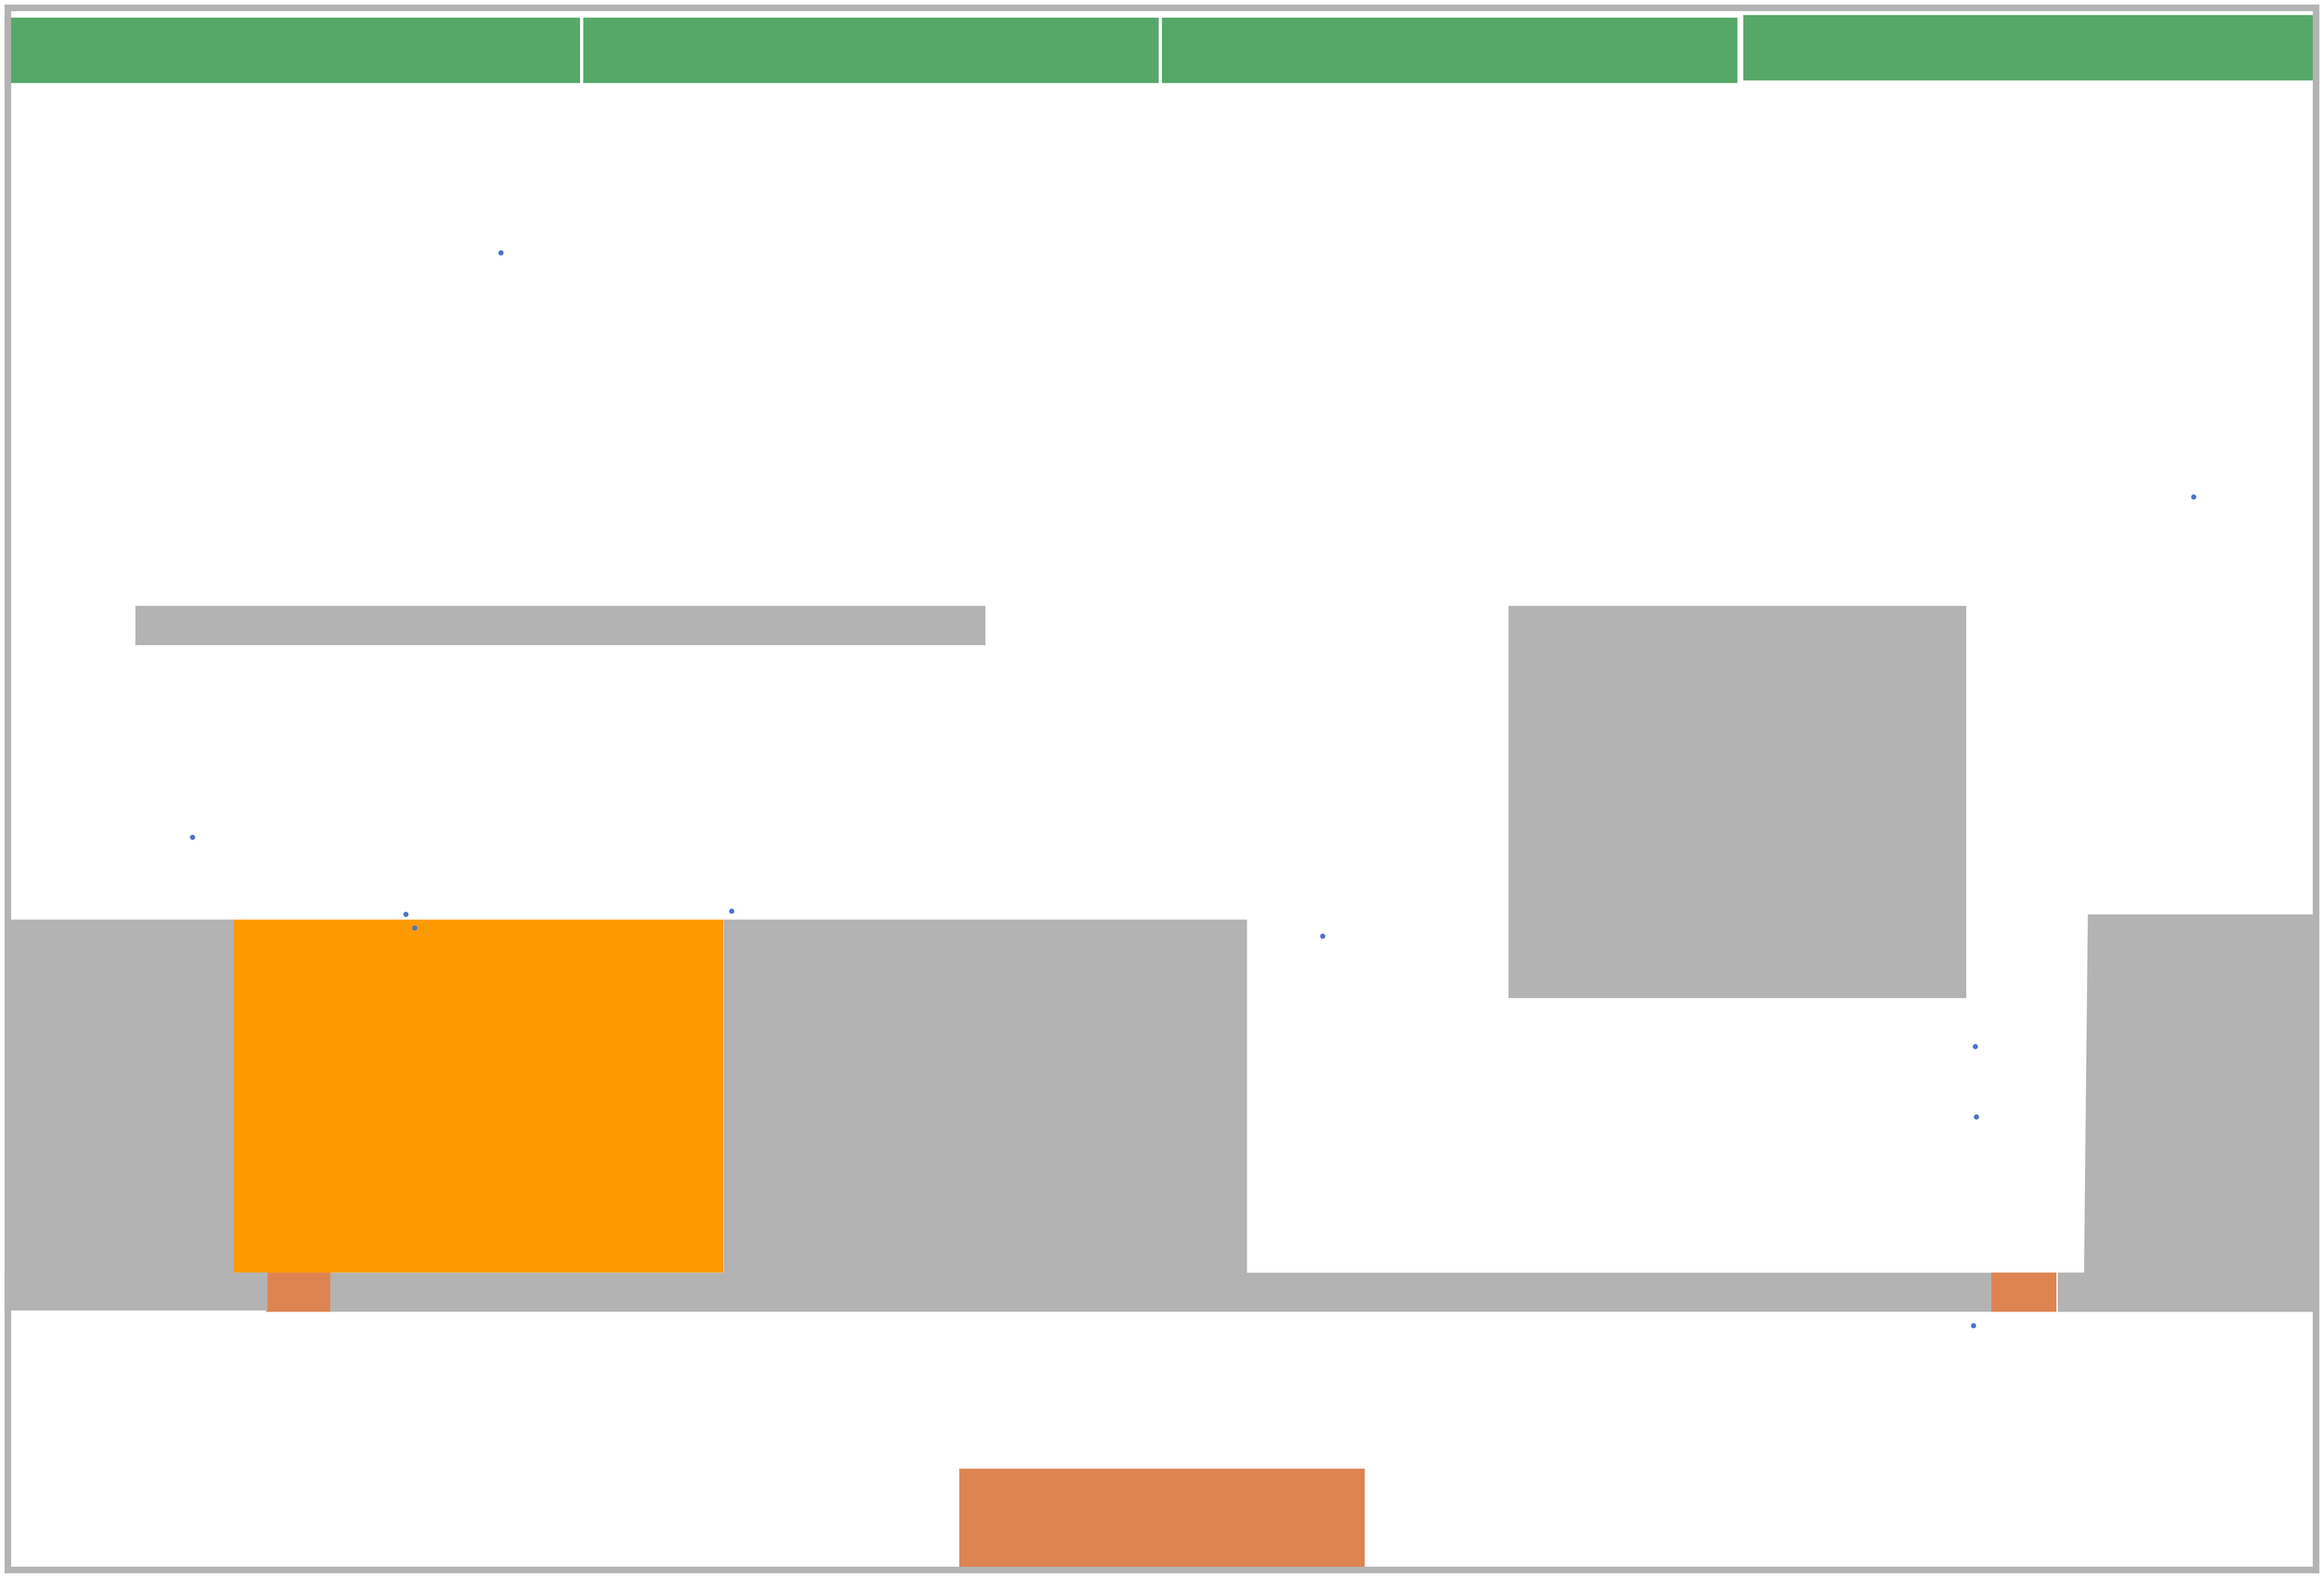
\begin{tikzpicture}
[x=1cm,y=1cm,
trajectory/.style={line width=1},
pedestrian/.style={circle, fill=AgentColor, minimum size=0.390000 cm},
walkdirection/.style={},
selected/.style={draw=magenta, line width=2},
group/.style={},
voronoi/.style={black, line width=1}
]
% Clipping
\clip (0.000000,0.000000) rectangle (177.000000,120.000000);
% Ground
\fill[white] (0.000000,0.000000) rectangle (177.000000,120.000000);
% Sources
\coordinate (Source1) at (22.000000,116.500000); % Centroid: Source 1
\fill[SourceColor] (0.000000,114.000000) to (44.000000,114.000000) to (44.000000,119.000000) to (0.000000,119.000000) to (0.000000,114.000000);
\coordinate (Source2) at (66.250000,116.500000); % Centroid: Source 2
\fill[SourceColor] (44.250000,114.000000) to (88.250000,114.000000) to (88.250000,119.000000) to (44.250000,119.000000) to (44.250000,114.000000);
\coordinate (Source5) at (110.500000,116.500000); % Centroid: Source 5
\fill[SourceColor] (88.500000,114.000000) to (132.500000,114.000000) to (132.500000,119.000000) to (88.500000,119.000000) to (88.500000,114.000000);
\coordinate (Source6) at (154.950000,116.700000); % Centroid: Source 6
\fill[SourceColor] (132.949997,114.199997) to (176.949997,114.199997) to (176.949997,119.199997) to (132.949997,119.199997) to (132.949997,114.199997);
% Targets
\coordinate (Target2001) at (88.500000,4.000000); % Centroid: Target 2001
\fill[TargetColor] (73.000000,0.000000) to (104.000000,0.000000) to (104.000000,8.000000) to (73.000000,8.000000) to (73.000000,0.000000);
\coordinate (Target2003) at (154.400000,21.500000); % Centroid: Target 2003
\fill[TargetColor] (151.899994,20.000000) to (156.899994,20.000000) to (156.899994,23.000000) to (151.899994,23.000000) to (151.899994,20.000000);
\coordinate (Target2002) at (22.500000,21.500000); % Centroid: Target 2002
\fill[TargetColor] (20.000000,20.000000) to (25.000000,20.000000) to (25.000000,23.000000) to (20.000000,23.000000) to (20.000000,20.000000);
% Target Changers
\coordinate (TargetChanger1) at (36.231244,36.500000); % Centroid: TargetChanger 1
\fill[TargetChangerColor] (17.498110,23.000000) to (54.964378,23.000000) to (54.964378,50.000000) to (17.498110,50.000000) to (17.498110,23.000000);
% Absorbing Areas
% Obstacles
\coordinate (Obstacle12) at (132.500000,59.000000); % Centroid: Obstacle 12
\fill[ObstacleColor] (115.000000,44.000000) to (150.000000,44.000000) to (150.000000,74.000000) to (115.000000,74.000000) to (115.000000,44.000000);
\coordinate (Obstacle13) at (42.500000,72.500000); % Centroid: Obstacle 13
\fill[ObstacleColor] (10.000000,71.000000) to (75.000000,71.000000) to (75.000000,74.000000) to (10.000000,74.000000) to (10.000000,71.000000);
\coordinate (Obstacle5009) at (8.900000,35.800000); % Centroid: Obstacle 5009
\fill[ObstacleColor] (17.500000,50.000000) to (0.300000,50.000000) to (0.300000,21.600000) to (17.500000,21.600000) to (17.500000,50.000000);
\coordinate (Obstacle2) at (9.850000,21.550000); % Centroid: Obstacle 2
\fill[ObstacleColor] (-0.400000,20.100000) to (20.100000,20.100000) to (20.100000,23.000000) to (-0.400000,23.000000) to (-0.400000,20.100000);
\coordinate (Obstacle3) at (88.395264,21.497158); % Centroid: Obstacle 3
\fill[ObstacleColor] (24.900000,20.007618) to (151.890518,20.007618) to (151.890518,22.986698) to (24.900000,22.986698) to (24.900000,20.007618);
\coordinate (Obstacle5002) at (75.000000,36.000000); % Centroid: Obstacle 5002
\fill[ObstacleColor] (95.000000,50.000000) to (55.000000,50.000000) to (55.000000,22.000000) to (95.000000,22.000000) to (95.000000,50.000000);
\coordinate (Obstacle4) at (166.925928,21.500000); % Centroid: Obstacle 4
\fill[ObstacleColor] (157.001205,20.000000) to (176.850647,20.000000) to (176.850647,23.000000) to (157.001205,23.000000) to (157.001205,20.000000);
\coordinate (Obstacle11) at (167.824784,36.159078); % Centroid: Obstacle 11
\fill[ObstacleColor] (159.000000,22.000000) to (176.500000,22.000000) to (176.500000,50.400002) to (159.300003,50.400002) to (159.000000,22.000000);
% Stairs
% Measurement Areas
% Voronoi Diagram (not enabled in config)
% Trajectories (not enabled in config)
% Agents
\node[pedestrian] (Pedestrian1) at (31.363804,49.358137) {};
\node[pedestrian] (Pedestrian2) at (100.790237,48.733225) {};
\node[pedestrian] (Pedestrian3) at (150.779272,34.905151) {};
\node[pedestrian] (Pedestrian5) at (14.373041,56.297253) {};
\node[pedestrian] (Pedestrian6) at (150.694434,40.289042) {};
\node[pedestrian] (Pedestrian7) at (150.559208,18.935348) {};
\node[pedestrian] (Pedestrian8) at (30.688679,50.401374) {};
\node[pedestrian] (Pedestrian9) at (55.600899,50.646533) {};
\node[pedestrian] (Pedestrian10) at (167.394340,82.330362) {};
\node[pedestrian] (Pedestrian11) at (37.957962,101.005995) {};
% Agent Ids (not enabled in config)
% Topography Boundary
\coordinate (BoundaryObstacle1) at (88.500000,0.250000); % Centroid: BoundaryObstacle -1
\fill[ObstacleColor] (-0.000100,0.500100) to (-0.000100,-0.000100) to (177.000107,-0.000100) to (177.000107,0.500100) to (-0.000100,0.500100);
\coordinate (BoundaryObstacle2) at (176.750000,60.000000); % Centroid: BoundaryObstacle -1
\fill[ObstacleColor] (176.499893,-0.000100) to (177.000107,-0.000100) to (177.000107,120.000099) to (176.499893,120.000099) to (176.499893,-0.000100);
\coordinate (BoundaryObstacle3) at (88.500000,119.750000); % Centroid: BoundaryObstacle -1
\fill[ObstacleColor] (177.000107,119.499901) to (177.000107,120.000099) to (-0.000100,120.000099) to (-0.000100,119.499901) to (177.000107,119.499901);
\coordinate (BoundaryObstacle4) at (0.250000,60.000000); % Centroid: BoundaryObstacle -1
\fill[ObstacleColor] (0.500100,120.000099) to (-0.000100,120.000099) to (-0.000100,-0.000100) to (0.500100,-0.000100) to (0.500100,120.000099);
\end{tikzpicture}
\end{document}
